 \documentclass[a4paper,12pt]{article}
\usepackage[utf8]{inputenc}
\usepackage{fullpage}
\usepackage{csquotes}
\usepackage[ngerman]{babel}
\usepackage{biblatex}
\usepackage{float}
\usepackage{graphicx}
\usepackage{subfigure}
\usepackage[format=plain,labelfont=bf,up]{caption}
\usepackage{hyperref}
\usepackage{booktabs}

\bibliography{expose}
\title{Gesture Control \\ VLC Remote Control für die Android-Plattform}
\author{Andreas Feldmann \\ Willi Schönborn}
\date{\today}
\begin{document}

\begin{figure}[H]
\centering

\includegraphics[width=0.5\textwidth]{beuth.eps}
\maketitle
\end{figure}

\section*{Projektidee}
Zur Zeit steigt die Nachfrage nach gut bedienbaren Streamingsystemen für den Heimbereich immer weiter an. Dabei wird nicht mehr nur auf die Installation und Wartbarkeit wert gelegt, sondern auch auf die Bedienbarkeit. Und doch können fest installierte Geräte mit Streamingsoftware meist nur über die eingesetzten Perephiegeräte gesteuert werden. \\
Da sich in den meisten dieser Haushalte auch ein mobiles Endgerät befindet, wäre eine Steuerung der Software über diese Technologie von Vorteil. Dabei spielt vor allem die Art der Steuerung eine wichtige Rolle. Der Benutzer soll nicht nur eine Oberfläche mit entsprechenden Schaltflächen vorfinden, sondern prägnante Gesten, die sich wie bei älteren Geräten vorfindbar, für eine simple Benutzung sorgen. Damit würde, wie bei klassischen TV-Geräten, eine Fernbedienung geschaffen die sich an den einprägsamen Bewegungen (in diesem Fall Gesten) orientiert. \\
Dieses Projekt soll sich mit der Umsetzung einer solchen Remotesteuerung von einem mobilen Endgerät aus, zur Streamingsoftware beschäftigen.

Es gibt freiverfügbare Apps mit ähnlichen Ansätzen. Am interessantesten ist wohl die \textit{Android VLC Remote} App \cite{android-vlc-remote}. Das größte Manko an Apps dieser Art ist, unserer Meinung nach, dass die Möglichkeiten des Smartphones nicht voll ausgereizt werden und damit die Möglichkeiten für eine größere Nutzerzufriedenheit nicht in dem Maße ausgeschöpft werden wie sie könnten.

\newpage
\section*{Konzept}

\subsection*{Gesten}
Alle letztendlich unterstützten Gesten sollen den folgenden Kriterien genügen. Durch die Einhaltung dieser Kriterien versprechen wir uns eine kurze Lernphase und damit extrem kleine Einstiegshürde für Nutzer der App.

\begin{itemize}
	\item \textbf{Erwartungskonform} \\
		Gesten wie Flick, Tap und Scale sind durch bestehende Apps bei vielen Nutzern bereits mental mit entsprechenden Funktionen verknüpft. Diese Erwartungshaltung sollte, sofern möglich, erfüllt werden.
	\item \textbf{Innovativ} \\
		Falls es für bestimmte Funktionen noch keinen Defacto-Standard gibt was eine Gestensteuerung betrifft, so sollen neue Gesten gefunden werden, die ggf. so noch nicht genutzt wurden. Wichtig dabei ist jedoch der nächste Punkt.
	\item \textbf{Intuitiv und nachvollzierbar} \\
		Bei neuartigen, ungewohnten oder seltenen Gesten sollte eine Funktion angestoßen werden, die sinnvoll zur entsprechenden Geste passt. Hier sind ggf. kleine A/B-Tests oder eng gefasste Fokusgruppen-Interviews sinnvoll.
\end{itemize}

Abbildung \ref{fig:gestures} zeigt einige Gesten die adhoc in Frage kommen sowie mögliche Funktionen, mit denen sie verknüpft werden könnten.

\begin{figure}[H]
\centering
\subfigure[Play/Pause]{
    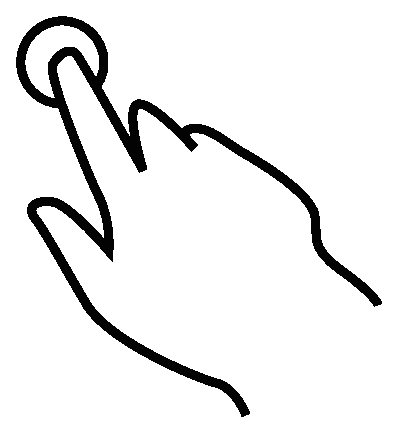
\includegraphics[width=0.2\textwidth]{one_finger_tap_gestureworks.eps}
}
\subfigure[Nächster Titel]{
    \reflectbox{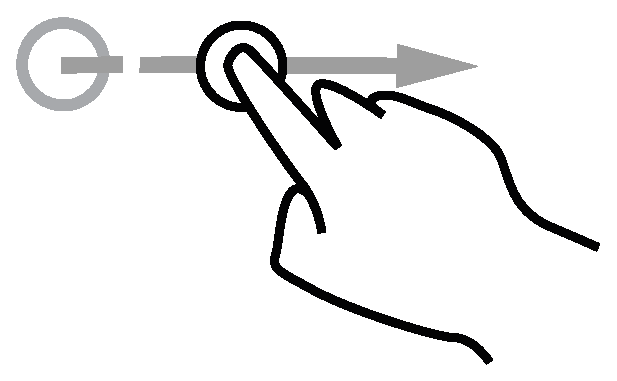
\includegraphics[width=0.35\textwidth]{one_finger_flick_gestureworks.eps}}
}
\subfigure[Vorheriger Titel]{
    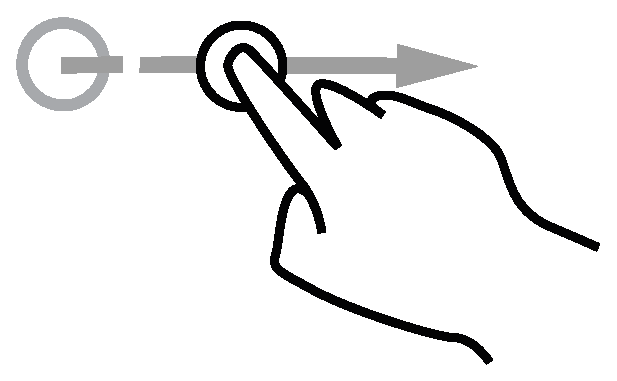
\includegraphics[width=0.35\textwidth]{one_finger_flick_gestureworks.eps}
}
\subfigure[Volume/Seek]{
    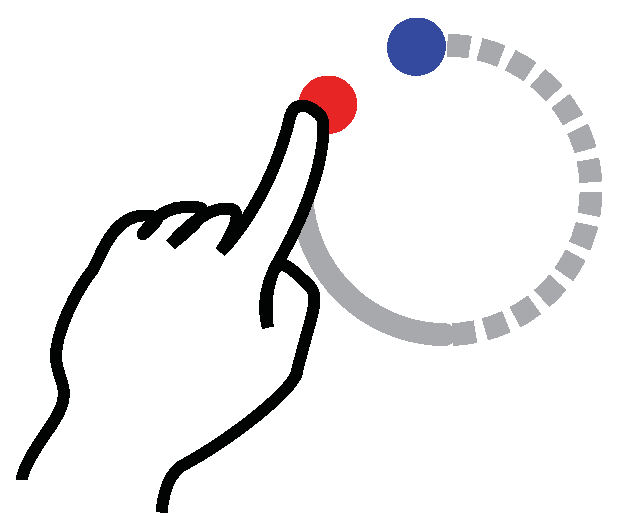
\includegraphics[width=0.3\textwidth]{stroke_shape_circle_gestureworks.eps}
    \label{fig:seek}
}
\subfigure[Vollbild]{
    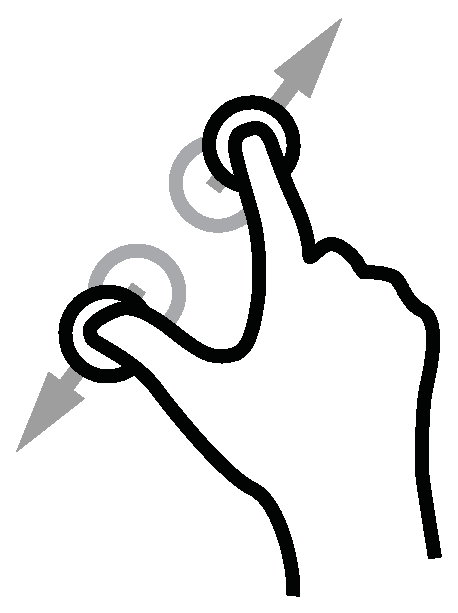
\includegraphics[width=0.2\textwidth]{two_finger_scale_gestureworks.eps}
}
\caption{Gesten}
\label{fig:gestures}
\end{figure}

\subsection*{Preview}

Ein optionales Zusatzfeature ist eine Seek-Funktion mit Preview, d.h. während die Seek-Geste (s. Abbildung \ref{fig:seek}) ausgeführt wird, soll ein Vorschaubild der aktuellen Suchposition innerhalb des Streams angezeigt werden. Abbildung \ref{fig:youtube} zeigt einen ähnlichen Ansatz des Youtube-Players. Hier wird auf einer Zeitleiste beim Mouse-Over ein entsprechender Tooltip angezeigt.

\begin{figure}[H]
\centering
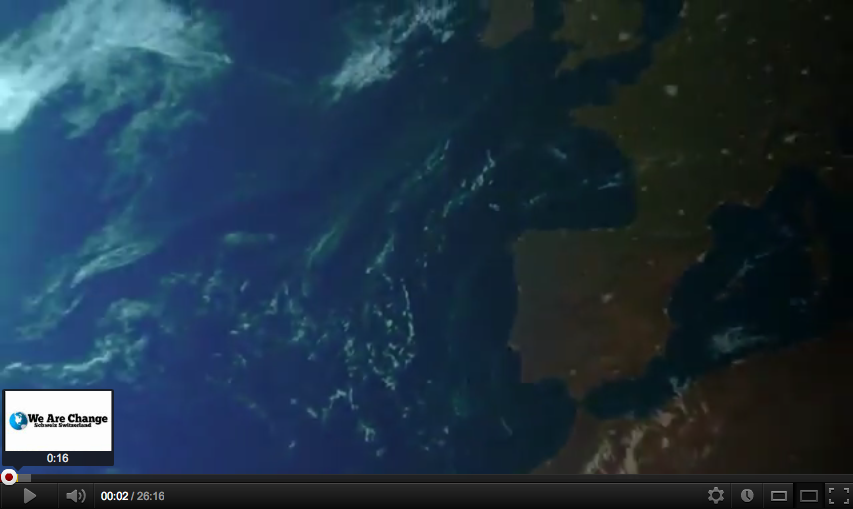
\includegraphics[width=0.75\textwidth]{youtube.png}
\caption{Youtube Preview Feature}
\label{fig:youtube}
\end{figure}

Die konkrete Darstellung muss natürlich für Smartphones separat konzipiert und entwickelt werden. Die besondere technische Herausforderung wird das Interagieren der Remote- und der Streaming-Schnittstelle sein, da die einzelnen Vorschaubilder über den Stream beschafft werden müssen.

\subsection*{Technologien}
Aus der Problemstellung wird zunächst ersichtlich, dass für die Umsetzung zwei verschiedene Komponenten betrachtenten werden müssen. Dies ist einerseits die Software, die zum Abspielen und Streamen der Medieninhalte zuständig ist, sowie anderseits das mobile Endgerät, das als Fernsteuerung dienen wird. \\
Für den Mediaplayer soll der VLC Media Player von VideoLan \cite{VLC} benutzt werden. Diese Software ist sowohl kostonlos, als auch für die gängigen Betriebssysteme verfügbar. Somit kann ein weiter Einsatz gewährleistet werden. Weiterhin besitzt der VLC eine HTTP-Schnittstelle \cite{VLC:WebInterface}, über die mittels \textit{controls} (Kontrollkommandos z.B. Start/Stop) und \textit{commands} (Einstellungen z.B. Lautstärke) der Player gesteuert werden kann \cite{VLC:HowTo}. \\
Auf der Seite des mobilen Endgeräts fiel die Wahl auf die verbreitete Android-Plattform \cite{Android}. Die Entwicklung von Software für dieses System ist ohne Einschränkung der Entwicklungsumgebung möglich und die Distribution ist konstengünstiger und einfacher, als seine Konkurrenzsysteme. Den Entwicklern liegen bereits Smartphones mit verschiedenen Android-Versionen vor, um den Echtzeitbetrieb für eine breite Verteilung zu entwicklen und zu testen.

\subsection*{Portierbarkeit}
Um die Ausbaufähigkeit der Anwendung sicherzustellen, wäre es wünschenswert, wenn es nur minimale Abhängigkeiten an den VLC Media Player als zu steuernde Software gibt. So wäre es in einer weiteren Ausbaustufe möglich dem Nutzer der App anzubieten diverse Video Player zu steuern, sofern sie unterstützt werden. Die Grundlage für diese Möglichkeit sollte dadurch sichergestellt werden, dass die eigentliche Kommunikation mit dem VLC Media Player innerhalb des Systems mithilfe sinnvoll definierter Schnittstellen gekapselt wird.

\newpage
\section*{Projektplanung}

Für die Realisierung dieses Projektes gilt folgender Meilensteinplan:

\subsection*{Version 1, \date{11.05.2012}}
\begin{itemize}
\item Evaluierung des VLC-HTTP-Schnittstellenumfangs
\item Layout aus den Vorgaben erstellen
\item Umsetzung der ersten Steuerungskomponenten
\end{itemize}

\subsection*{Version 2, \date{08.06.2012}}
\begin{itemize}
\item Implementierung der weiteren Steurungsfunktionen
\item Evaluierung der Übermittlung von Metadaten an das Mobilgerät
\item Implementierung der Previewfunktionalitäten
\end{itemize}

\subsection*{Version 3, \date{03.07.2012}}
\begin{itemize}
\item Fertigstellung der Funktionalitäten
\item Qualitätssicherung
\item Installation auf mobilen Testgeräten
\end{itemize}

\section*{Projektaufteilung}
Die Entwicklung des Projektes wird zu gleichen Teilen auf die Entwickler Schönborn und Feldmann getragen, wobei die Zuständigkeiten wie folgt verteilt werden:

\begin{table}[h!b!p!]
\begin{tabular*}{\textwidth}{ l l l l }
	\toprule
	\textbf{Aufgabe} & \textbf{Version} & \textbf{Entwickler} \\
	\midrule
	Gestenentwicklung & 1 & Willi Schönborn  \\ 
	User Interface & 1, 2 & Willi Schönborn \\
	Gestenerkennung & 2 & Willi Schönborn \\
	VLC HTTP Interface & 1, 2 & Andreas Feldmann \\
	Remote Control Interface & 1, 2 & Andreas Feldmann \\
	Streaming & 2 & Andreas Feldmann \\
	\bottomrule
\end{tabular*}
\end{table}

\newpage
\nocite{*}
\printbibliography

\listoffigures

\end{document}

